\chapter{Experimentación}

\section{Beacons y configuración}

Los beacons utilizados corresponden a beacons de la marca Kontakt, y el numero es 8, sin embargo, no son todos iguales. Esto ayuda a comprobar que tan efectivo es utilizar distintos modelos, ya que en entornos reales, por ejemplo en una mina, es sumamente importante contar con beacons bluetooth que se adapten al espacio físico en donde son dispuestos, por ejemplo si es necesario instalarlos en una oficina, los beacons convencionales funcionan de buena manera, sin embargo en ambientes hostiles como lugares con polvo o de difícil acceso, es necesario contar con beacons preparados para estas dificultades, los cuales tengan baterías de larga duración, sean anti polvo y agua, entre otras características. A continuación se muestra el resumen de los beacons utilizados:

\begin{enumerate}
\item \textbf{Beacon: } Beacon mas popular y de menores prestaciones. Es el clásico Beacon vendido por la compañía Kontakt. Posee una batería con duración de hasta 48 meses y un rango de 70m. Se utilizan 4 unidades.

\item \textbf{Beacon Pro: } Beacon con mas funciones de seguridad, ahorro de bateria, sensores de luz y a prueba de agua. Hasta 60 meses de bateria y rango de 70m. Se utilizan 2 unidades.

\item \textbf{Tough Beacon: } Hasta 24 meses de batería y rango de 70m. A prueba de polvo y agua. Especialmente diseñado para condiciones extremas.


\end{enumerate}

Cabe destacar que las caracteristicas basicas del \textit{Hardware} de cada beacon son las presentes en la comparativa realizada en la sección \ref{sec:seleccion}.

Foto beacons.

Lo siguiente es definir la configuración de cada Beacon. Los parámetros mas relevantes en este caso serian el \textit{TX Power} y el \textit{Beacon Interval}. En un despliegue real, lo mas relevante es disminuir los costos, que en este caso están asociado a las baterias o mas bien al cambio de estas a lo largo del tiempo. Estos dos parametros son importantes para la localización indoor, ya que el TX Power define la potencia de salida de cada Beacon y el intervalo corresponde a cada cuanto un beacon envía un mensaje a los dispositivos bluetooth cercanos. 

El valor de Tx Power afecta principalmente a tres factores claves, estos son el rango de la señal, es decir, la distancia maxima alcanzada; el segundo corresponde a la estabilidad de la señal y finalmente la bateria, aunque este ultimo factor es mayormente influenciado por el intervalo.

En terminos simples, TX Power representa que tan poderosa es la señal transmitida por los beacons en dBm y corresponde a un numero dentro del rango 0-7, donde 0 es menos poderoso y 7 el mas poderoso.Es claro que mientras mas poderoso es la señal, mayor rango alcanza y mas estable es la señal, sin embargo el consumo de energia aumenta significativamente. Para determinar el parametro TX power entonces es necesario tener en cuenta estos factores. Para el caso del posicionamiento indoor, es claro que el rango debe ser maximo, ya que de esta forma la señal de cada Beacon puede alcanzar a la gran parte de los usuarios de la zona. El otro punto significativo es establecer que tan seguido es necesario cambiar las baterias. Este punto es relevante para despliegues a gran escala y depende en gran medida de las organizaciones interesadas en desplegar un sistema de este tipo. Finalmente, es importante considerar la interferencia subyacente debido al entorno, por ejemplo objetos contundentes o multiples personas, en este caso se requiere una señal mas potente para cortar de esta forma la interferencia y pasar a traves de esta. Por los motivos declarados anteriormente se decide utilizar un TX Power igual a 7, o equivalentemente 4 dBm.

Con respecto al intervalo utilizado, es un parámetro de mucho mayor relevancia que el TX Power para el tipo de problema a resolver. Esto se debe principalmente a que el intervalo corresponde a que tan frecuente es transmitido un paquete desde un Beacon a un dispositivo móvil. Considerando que el posicionamiento debe ser lo mas cercano a  tiempo real, la información debe ser suministrada lo mas rápidamente posible. El intervalo es medido en milisegundos, y como es esperable, mientras mas pequeño el intervalo, mas recurrente es la comunicación pero mayor es el consumo de batería. A pesar de que el intervalo sea muy pequeño, muchas veces los sistemas operativos no son capaces de recibir tan rápidamente estas señales, debido a limitaciones de seguridad u otras configuraciones del fabricante como es el caso de Apple. En Android estas limitaciones no existen y por lo tanto puede recibir todas las señales, pero esto afecta de forma significativa la batería del teléfono. Por otra parte, mientras menor es el intervalo, mayor es la estabilidad de la señal, ademas el intervalo afecta significativamente a el posicionamiento en interiores, debido a que mientras mas rápido se mueve un usuario, si el intervalo es demasiado alto, su posición sufrirá saltos o cortes que no muestran realmente la ruta de desplazamiento. Si el intervalo es pequeño, puede detectar mas fácilmente la posición del usuario en cada momento con precisión de unos pocos centímetros. La  ejemplifica esta situación:


\begin{figure}[ht!]
\centering
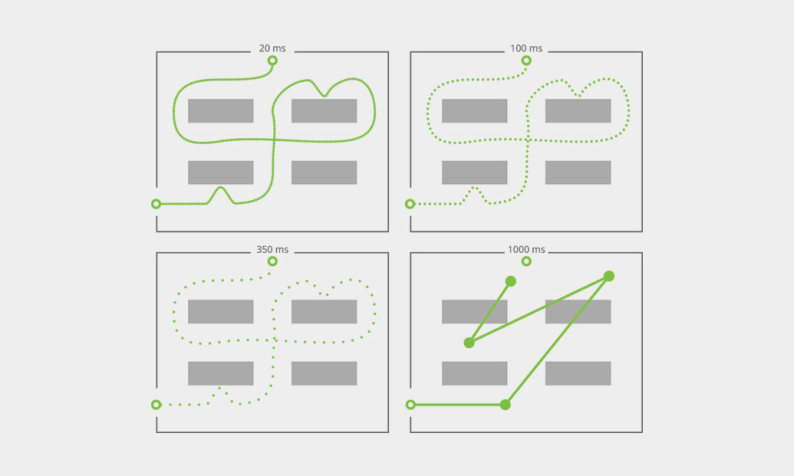
\includegraphics[width=.6\textwidth]{figures/interval.jpg}
\caption[abs]{Posicionamiento indoor con diferentes intervalos de aviso en mili segundos\\
{\scriptsize (Fuente: \cite{interval})}}
\label{fig:intervalo}
\end{figure}

Por lo anterior, es claro que los parámetros seleccionados deben ser el mayor valor posible para el TX Power correspondiente a 7, y un valor del intervalo igual a 100ms. Para configurar estos parámetros, Kontakt dispone de una aplicación para dispositivos Android. La \autoref{fig:kontaktapp1} y \ref{fig:kontaktapp2} muestran como han sido configurados los Beacons. Esta configuración es idéntica para todos los beacons utilizados.


\begin{figure}[ht!]
\centering
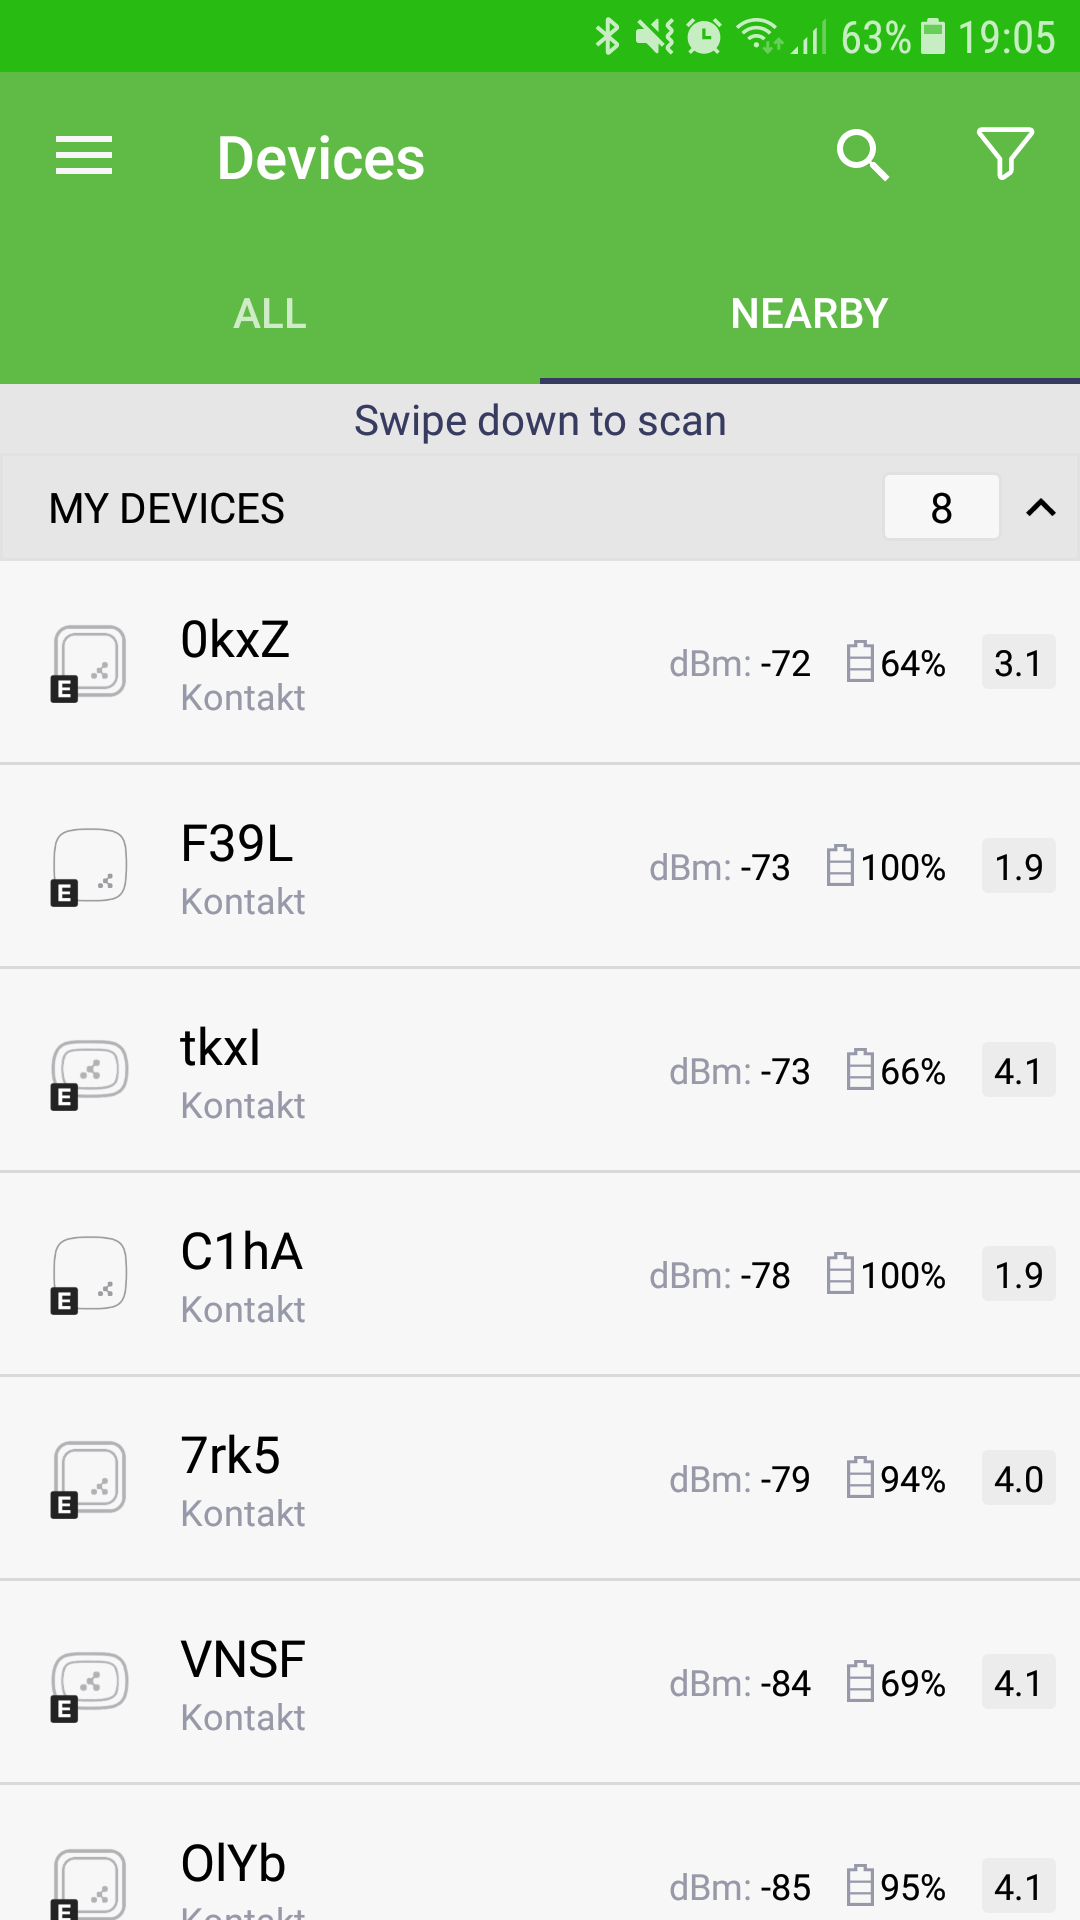
\includegraphics[width=.3\textwidth]{figures/kontaktapp1.png}
\caption[abs]{Listado de los beacons encontrados para su posterior configuración\\
{\scriptsize (Fuente: Elaboración Propia)}}
\label{fig:kontaktapp1}
\end{figure}

\begin{figure}[ht!]
\centering
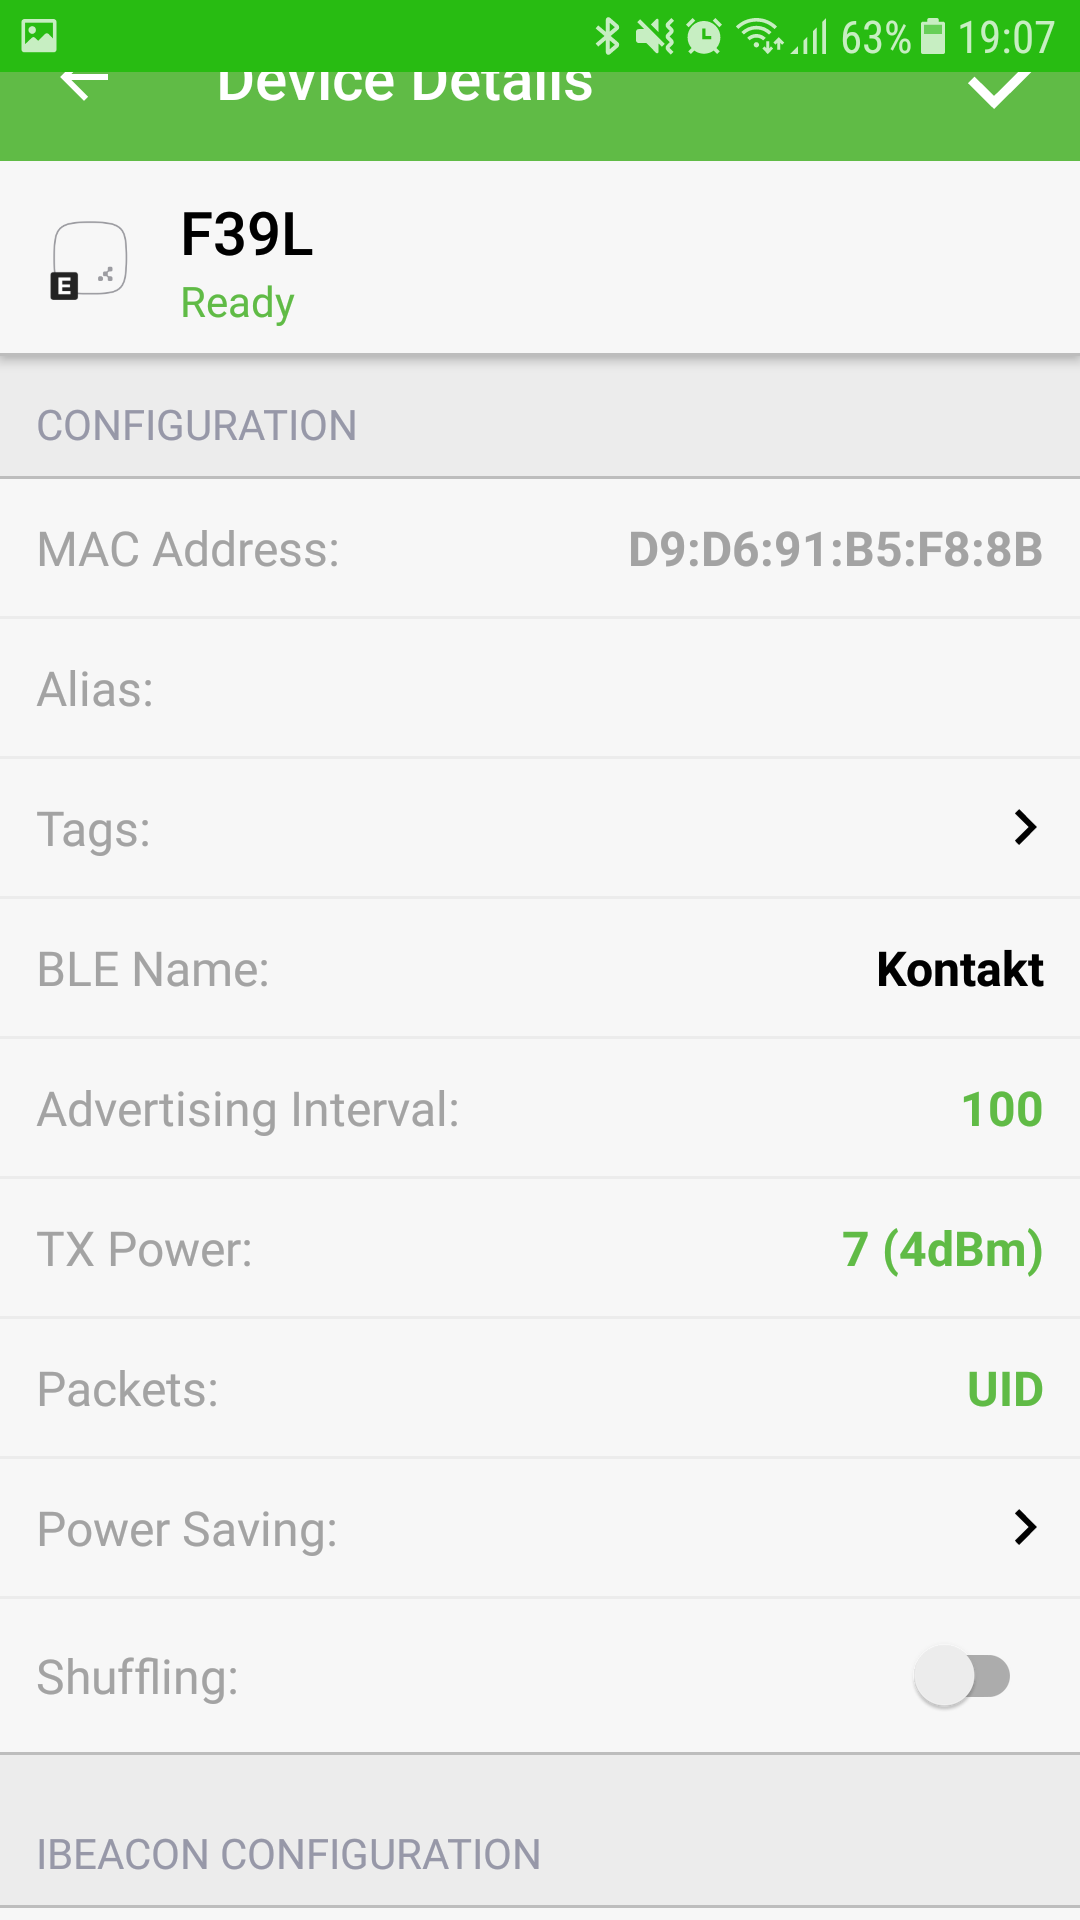
\includegraphics[width=.3\textwidth]{figures/kontaktapp2.png}
\caption[abs]{Configuración que ejemplifica los valores definidos para TX Power y el intervalo de transmisión\\
{\scriptsize (Fuente: Elaboración Propia)}}
\label{fig:kontaktapp2}
\end{figure}

Ademas, los protocolos utilizados son UID de Eddystone por su flexibilidad y transversalidad para los múltiples dispositivos móviles existentes en el mercado.

\section{Lugar de experimentacion}

Para realizar los experimentos, se decide utilizar un lugar en donde las condiciones sean adversas y cambiantes, debido al alto transito de objetos y ademas no se presenten señales GPS. Por lo anterior, se decide utilizar el estacionamiento subterráneo de la universidad Técnica Federico Santa Maria, Campus San Joaquin, ubicado en Vicuña Mackenna 3939. Las dimensiones constan de $144.75m$ de largo y $36m$ de ancho. La \autoref{fig:estSubterraneo} muestra el plano del estacionamiento a escala.

\begin{figure}[ht!]
\centering
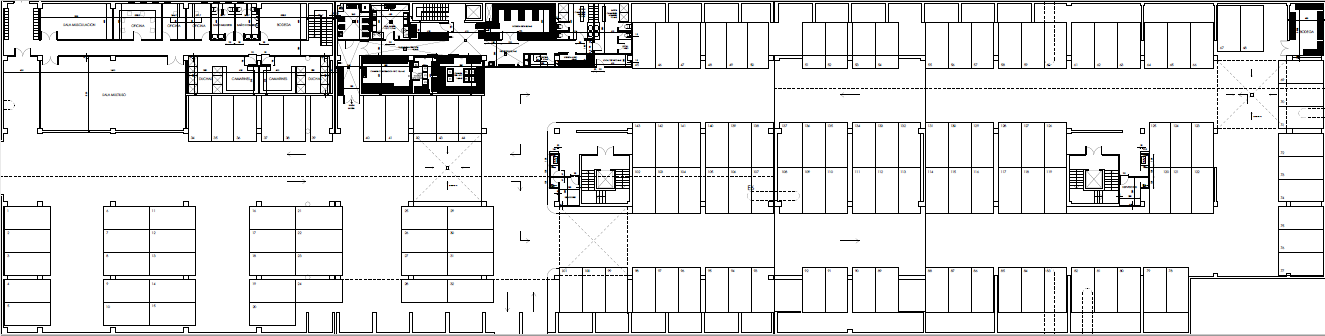
\includegraphics[width=.6\textwidth]{figures/estSubterraneo.png}
\caption[abs]{Plano del estacionamiento subterraneo de la Universidad Federico Santa Maria\\
{\scriptsize (Fuente: Elaboración Propia)}}
\label{fig:estSubterraneo}
\end{figure}

Este lugar es ideal para realizar pruebas, ya que presenta interferencia debido a los vehiculos en transito y la disposicion de los objetos es cambiante. Ademas, se pueden obtener mediciones con ruido producto de la reflexion de las ondas, lo que pone a prueba a los algoritmos de clasificación para detectar estos patrones. 

\begin{figure}[ht!]
\centering
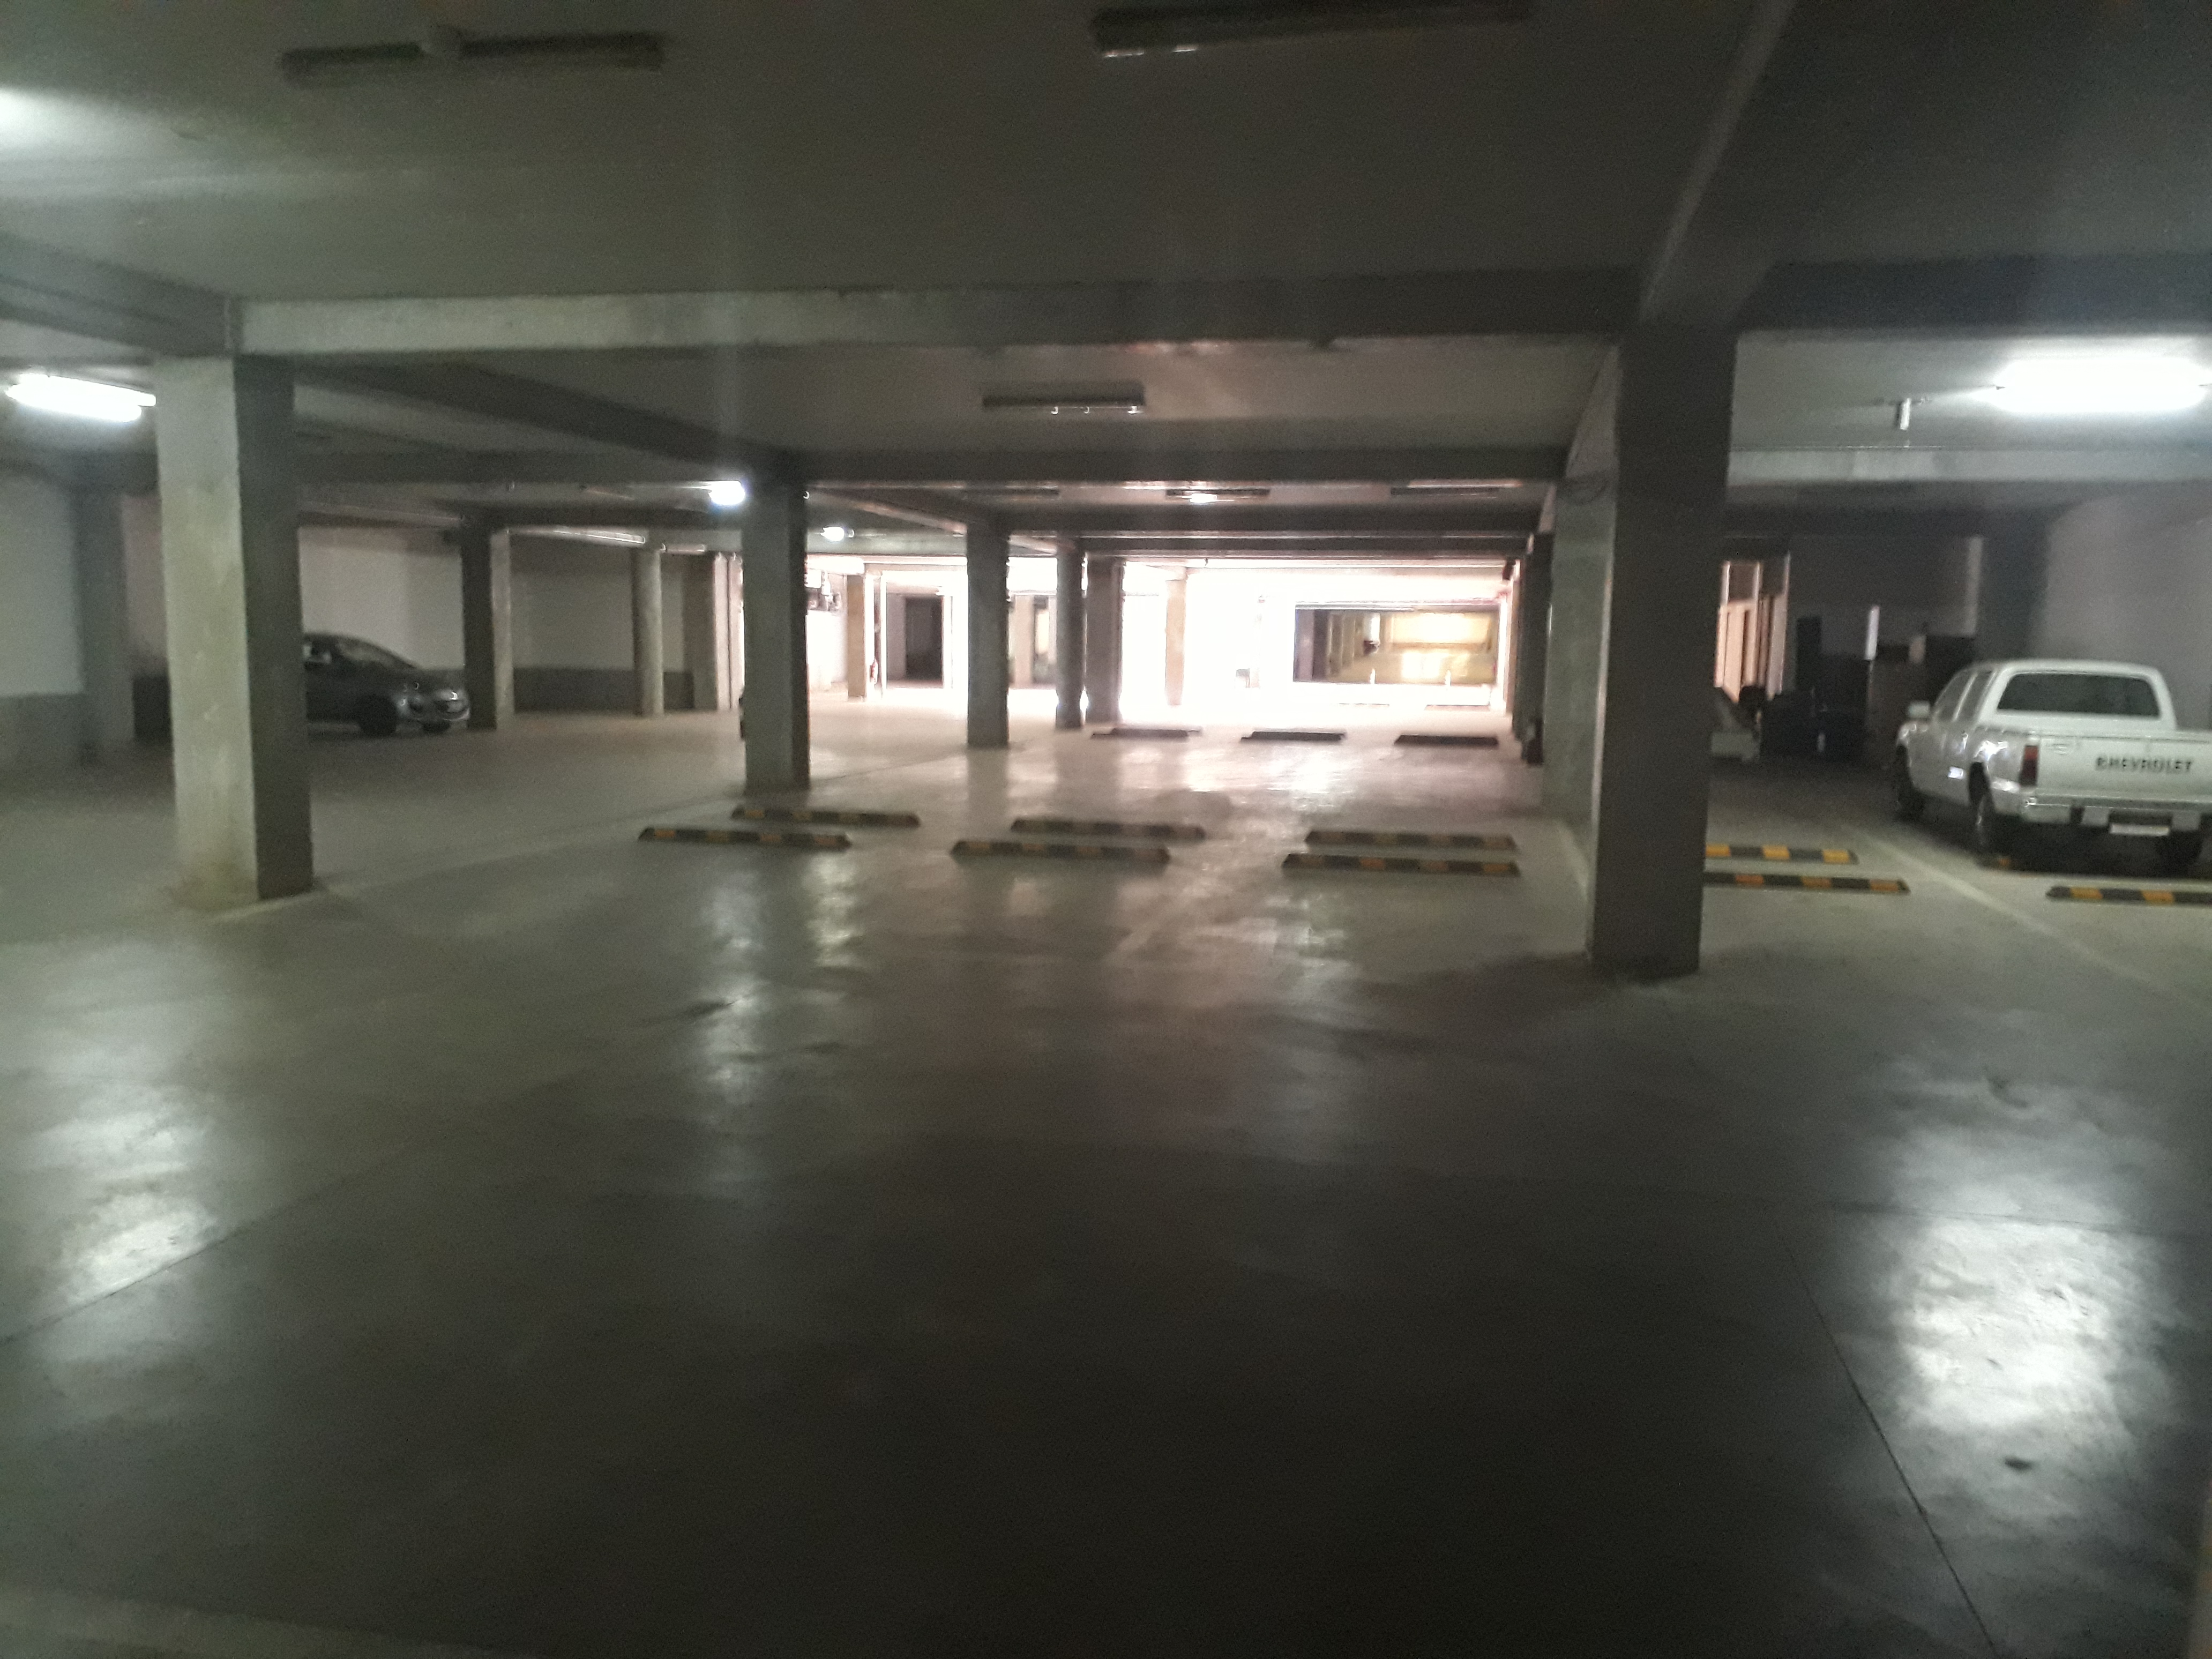
\includegraphics[width=.6\textwidth]{figures/estReal.jpg}
\caption[abs]{Fotografía del espacio de experimentación real, correspondiente al estacionamiento subterraneo\\
{\scriptsize (Fuente: Elaboración Propia)}}
\label{fig:estReal}
\end{figure}


\section{Software Utilizado}

\subsection{Descripción de la aplicación}

La aplicación desarrollada es construida para el sistema operativo Android. Para su desarrollo se utiliza Android Studio \footnote{\url{https://developer.android.com/studio/index.html}}, es IDE oficial para el desarrollo de aplicaciones nativas. El numero de compilación corresponde a $3.0.1$. La selección de este sistema operativo es debido a su fácil acceso y prácticamente ningún costo debido a licencias, ya que es basado en linux por lo que su desarrollo es gratuito, al igual que la distribución de aplicaciones, por lo que es mucho mas efectivo para el desarrollo de una aplicación de prueba bajo un entorno controlado.

Los requisitos básicos de la aplicación construida son los siguientes:

\begin{itemize}
\item Mostrar el plano del lugar de experimentación, el cual funciona como base para posicionar los demás elementos.

\item Permitir la adición de nuevos dispositivos Beacons con su respectivo marcador. Para ello debe detectar automáticamente el beacon mas cercano y sugerir este para su inserción en el mapa.

\item Permitir la captura de datos, es decir, los nuevos fingerprints, en donde el usuario es quien provee la posición exacta y la aplicación mide los valores RSSI durante un periodo de tiempo, para posteriormente almacenarlos en la base de datos. 

\item Modificar los valores de intervalo y el numero de mediciones en cada punto, el cual puede también definirse en periodo de tiempo.

\item Tener una base de datos \textit{SQLite}, la cual permite la persistencia de los datos. También se debe poder transformar esta base de datos a un archivo CSV.

\item Para la etapa online, debe permitir seleccionar el algoritmo a utilizar y mostrar en tiempo real la posición del usuario según el algoritmo usado. Por otra parte, debe guardar estos resultados en un archivo de texto para su posterior análisis.



\end{itemize}

La aplicación construida consta de 3 secciones principales las cuales ayudan a todas las etapas del modelo fingerprint, estas son \textbf{Offline}, \textbf{Online} y \textbf{Configuración}. Estas son descritas a medida que se desarrolla el proceso de la experimentación.


\subsection{scikit-learn}

Para la elaboración de modelos de clasificación, una de las librerías mas utilizadas es scikit-learn o tambien conocida como SKlearn \cite{scikit-learn}, la cual es una completa API para elaborar y realizar maquetas de machine learning. Su core esta basado en python y para su uso se utiliza el siguiente entorno de desarrollo:

\begin{itemize}
\item Anaconda 1.6.2
\item Jupyter Notebook 5.0.0
\item scikit-learn 0.18.2
\item Python 3.6.1
\end{itemize}

Las principales ventajas de utilizar SKlearn son obtener modelos simples y eficientes, que estan muy avanzados y que presentan una comunidad dedicada a su correcto funcionamiento. Ademas esta construida sobre 3 de las librerías mas utilizadas en Python en el contexto de desarrollo científico, como son NumPy, SciPy y Matplotlib. Por otra parte su licencia es de codigo abierto, por lo que cualquiera puede utilizar y modificar el código sin restricciones.

A pesar que en este caso solo se utilizara para los algoritmos de clasificación, PCA y gráficos, también presenta herramientas que agilizan el desarrollo como por ejemplo lectura de archivos, funciones de normalizacion establecidas, funciones de puntuación o accuracy, pre procesamiento de datos, entre otras. También sirve como herramienta de regresión, minería de datos y análisis de datos.

\section{ Tensorflow}

A pesar que SKlearn presenta tantas ventajas para el desarrollo agil de modelos de maquinas de aprendizaje, no es tan bueno en redes neuronales, y no implementa la mayor parte de los algoritmos modernos en este campo. Esto se debe principalmente a que todo el core de SKlearn es python, y se vuelve sumamente lento para entrenar este tipo de redes, sobre todo redes profundas. Para resolver este problema, se decide utilizar Tensorflow \cite{tensorflow2015-whitepaper}, un completo framework de desarrollo de Google, que con respecto a SKlearn es mucho menos intuitivo y de fácil uso al usuario final, ya que su programacion es de mucho mas bajo nivel y requiere conocimiento avanzado de los algoritmos que se quieren implementar.  Mucha veces se describe como las piezas fundamentales para la creacion de algoritmos de maquinas de aprendizaje, como si fueran Legos, no asi SKlearn, el cual ya esta todo listo, solo debe ser utilizados y configurar los parametros de los algoritmos.

Tensorflow es una biblioteca de código abierto y su principal ventaja es que a pesar que la parte superior esta basada en python, esta se comunica internamente a código compilado en C++, lo cual lo vuelve sumamente eficiente. Ademas, por la forma en que Tensorflow representa los datos, es decir, tensores o arreglos multidimensionales, y las operaciones referentes a grafos sin estado que transforman estos tensores, lo vuelve increiblemente rapido para entrenar y desplegar, incluso presenta API para dispositivos moviles en Java, C++ y GO, en donde solo se porta el grafo construido y se puede realizar inferencia en equipos de muy pocos recursos, lo que lo vuelve una alternativa ideal para desarrollar redes neuronales profundas, utilizando  pocos recursos en el sistema operativo Android. A pesar de que presenta operaciones de bajo nivel, igualmente tiene disponible la opcion de API de alto nivel, como por ejemplo implementar redes convolucionales o redes profundas en un par de lineas de codigo Python, conocidos como estimadores de alto nivel.

Finalmente tensorflow basa todo su procesamiento en el grafo computacional mencionado anteriormente, el cual consiste en una serie de operaciones de tensores dispuestos en un grafo de nodos. Luego de que se arma este grafo de operaciones, se puede entrenar mediante las operaciones incluidas en tensorflow, llamados optimizadores, como lo son gradiente descendente. El paso final es utilizar este grafo computacional para probar los modelos y utilizarlos en despliegues reales.


\section{Recolección de fingerprints}


Con todo lo anterior en cuenta, es necesario definir que tipo de dispositivo móvil y sistema operativo se utilizara para colectar los datos en cuestión, que finalmente se transformaran en fingerprint dando lugar al radiomap. En este caso, el dispositivo a utilizar es un dispositivo Samsung Galaxy J7 Prime, que dentro de sus prestaciones posee una CPU Octa-core 1.6 GHz Cortex-A53, una GPU Mali-T830 MP1, 3GB de memoria ram interna y el tipo de Bluetooth corresponde a 4.1 LE. Con respecto a su sitema operativo, es Android 7.0 Nougat el cual no presenta limitaciones en la lectura de las señales Bluetooth por lo que puede recepcionar las señales tan rápido como estas son emitidas.

Definido esto, lo siguiente establecer la forma en que deben ser posicionados los beacons y ademas como funciona la recolección de fingerprints como tal. Para el posicionamiento de los Beacons, se decide utilizar una estrategia de grilla, esto es, ubicarlos de manera equidistante en las esquinas del plano. Ademas, para este trabajo se debe considerar que el plano completo no fue inspeccionado debido a que la densidad de los beacons seria muy baja para lograr óptimos resultados, por lo que finalmente se decide utilizar los 8 beacons en un área reducida del estacionamiento y ubicar cada beacon a una distancia de 16 metros a sus vecinos adyacentes formando esta especie de grilla. Finalmente, el área efectiva a utilizar se calcula según las dimensiones de 16 metros de ancho por 44 metros de largo, con lo que se obtiene un área de $704m^2$. Cabe destacar que un par de beacons fueron ubicados respecto a sus vecinos a una distancia de 12 metros y no 16, debido a la disposición del estacionamiento. 

Con respecto al punto de recolección de fingerprints, se desarrolla una aplicación para el sistema operativo Android, y se decide utilizar una grilla para los puntos de medición o referencia de 4 metros por 4 metros, es decir, cada punto de medición esta en medio de cada celda de esta grilla, consiguiendo de esta manera un total de 44 puntos de referencia. La \autoref{fig:deployBeacons} muestra esta situación.


\begin{figure}[ht!]
\centering
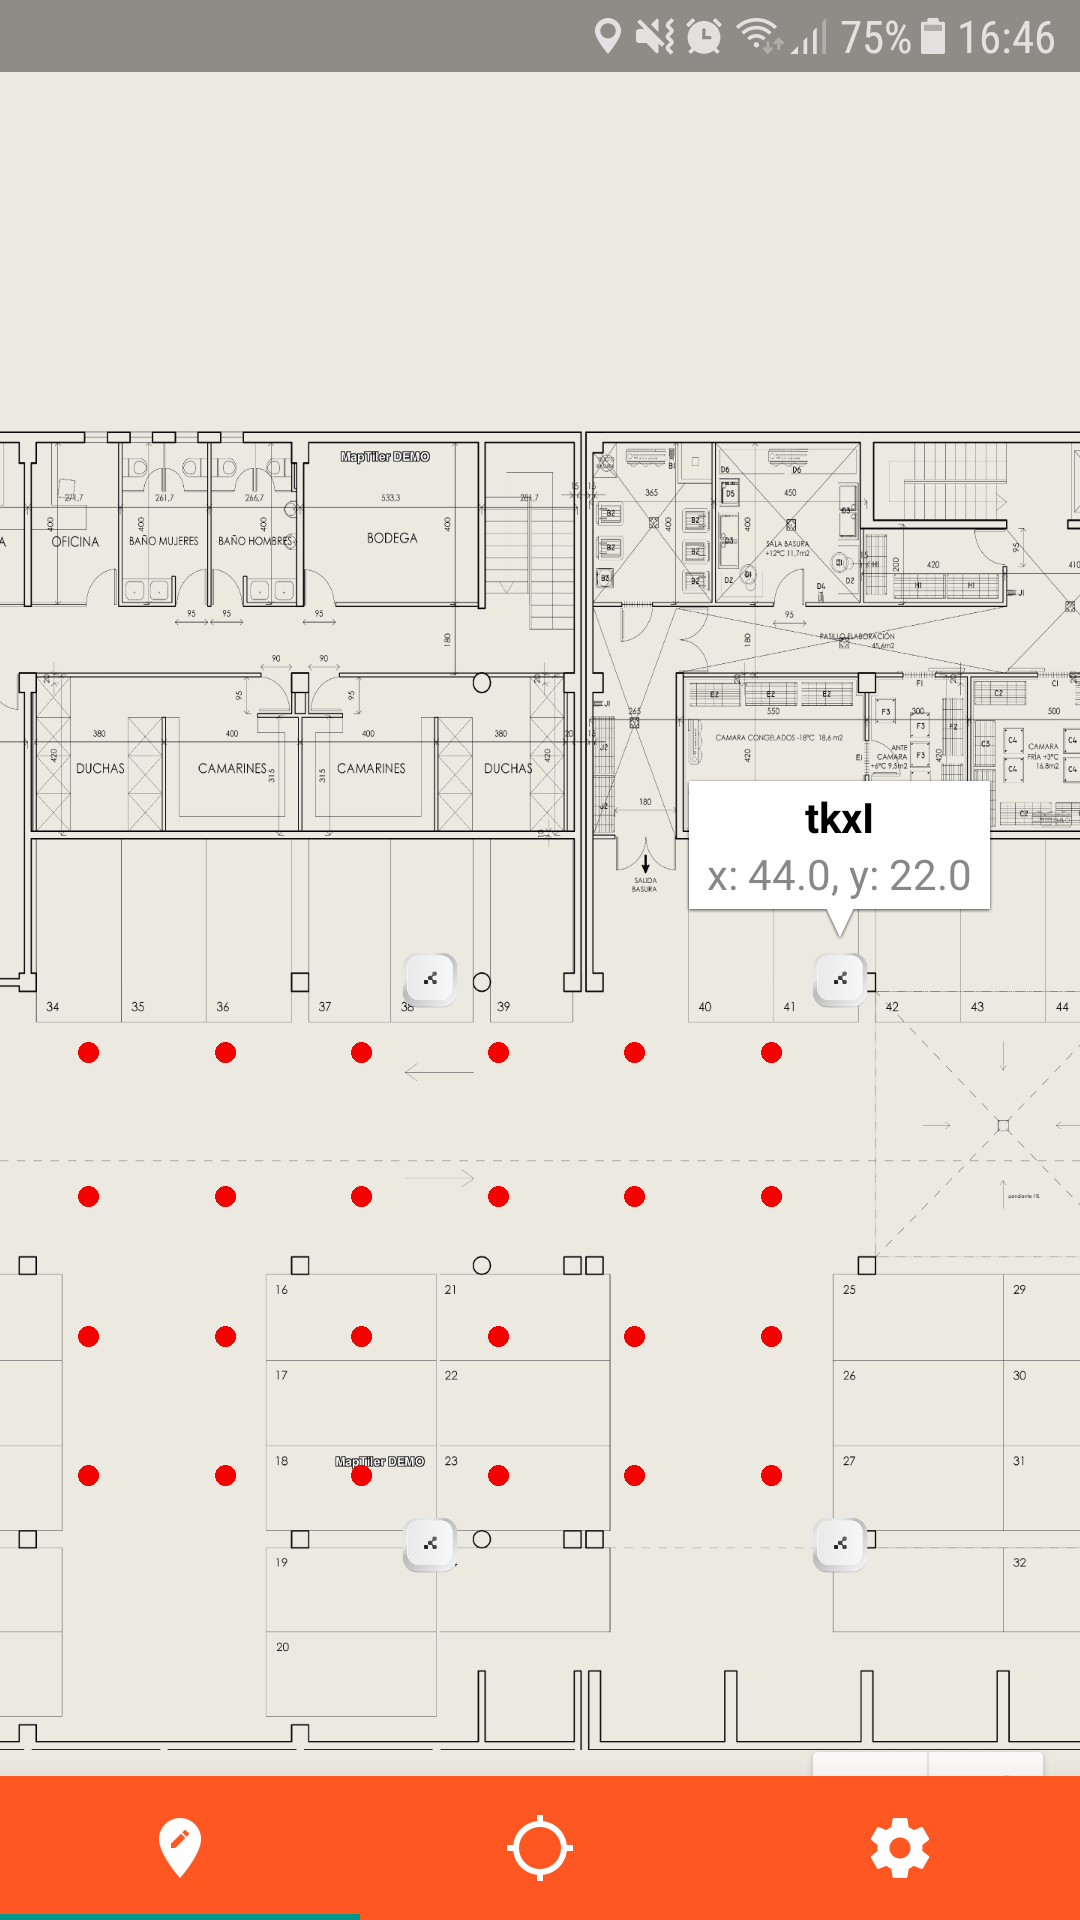
\includegraphics[width=.3\textwidth]{figures/deployBeacons.png}
\caption[abs]{Disposicion de beacons y puntos de referencia dentro de la grilla, utilizando la aplicacion Android\\
{\scriptsize (Fuente: Elaboración Propia)}}
\label{fig:deployBeacons}
\end{figure}

La aplicación consta de una sección offline, en donde se pueden incorporar nuevos Beacons a la base de datos \textit{sqlite}(base de datos por defecto en dispositivos Android), ademas de poner realizar  la captura de datos o fingerprints, definiendo la ubicación actual según algún patrón o posición exacta. Otro punto importante a considerar es el numero de fingerprints a obtener en cada punto de referencia. Considerando el intervalo de emisión de cada Beacon, es necesario establecer un tiempo alto para notar cambios en el lugar de experimentación, por lo que se define una ventana de tiempo de 5 minutos en cada punto de referencia. Sin embargo, para obtener mejores resultados y en vista y considerando que las maquinas de aprendizaje aprenden de mucho mejor manera con datos variados, se decide inspeccionar y recolectar datos a través de diferentes días, con el objetivo de que sea mas fácil para los algoritmos encontrar patrones eventualmente.

Una vez recolectados los datos, se obtiene una base de datos \textit{SQLite} con figerprints, la cual presenta 132000 registros, en donde los dos primeros campos representan la posicion de X y la posicion de Y respectivamente, y los siguientes 8 campos corresponden a los Beacons detectados con su respectiva intensidad de la señal o RSSI. Un punto importante a definir es que valor asignar a los beacons que no han sido detectados, en este caso y como el valor RSSI no puede ser mayor a cero, se decide asignar un valor de 100 dBm como un identificador de que no se ha detectado señal.

Con esta base de datos es posible construir otros tipos de archivos, que resuman todos los fingerprints detectados. Esto se realiza ya que para los algoritmos de machine learning existen muchas mas librerías dedicadas a leer datos en formatos mas convencionales como TXT o CSV. Por lo mismo, en la aplicación se define una sección de configuración para transformar y almacenar esta base de datos en formato CSV o \textit{comma-separated values}.  La \autoref{fig:configApp} muestra esta pestaña de configuracion, incluyendo el numero de mediciones y las opciones de exportar la base de datos, transformarla a CSV o eliminarla.

\begin{figure}[ht!]
\centering
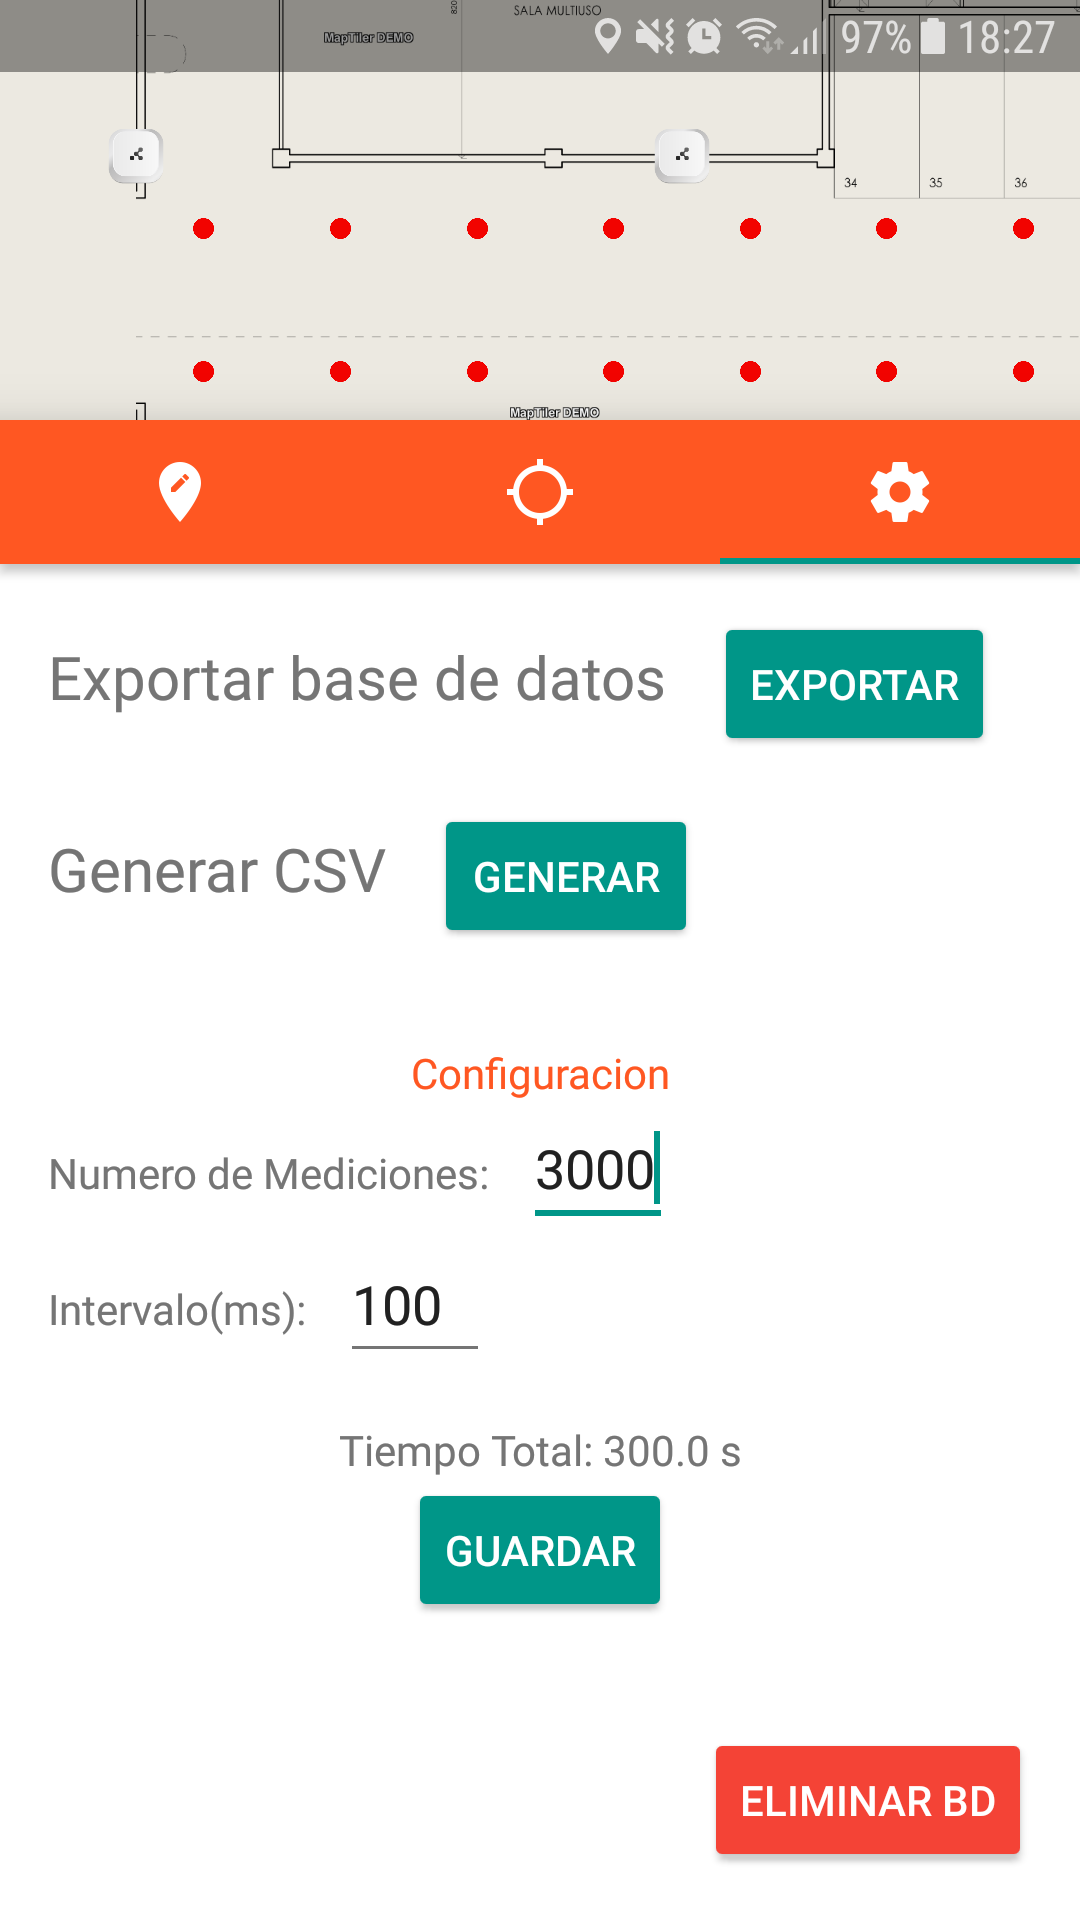
\includegraphics[width=.3\textwidth]{figures/configApp.png}
\caption[abs]{Pestaña de configuración de la aplicación Android, donde se puede configurar el tiempo y exportar la base de datos a CSV\\
{\scriptsize (Fuente: Elaboración Propia)}}
\label{fig:configApp}
\end{figure}


Un ejemplo del archivo CSV obtenido se presenta en la \autoref{fig:ejemploCSV}


\begin{figure}[ht!]
\centering
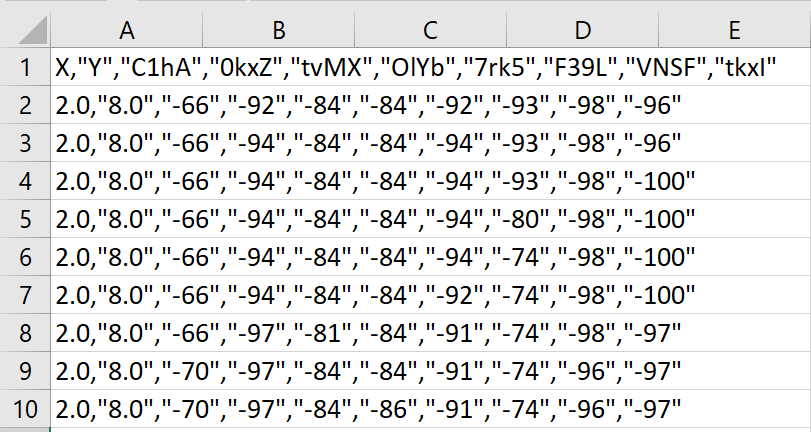
\includegraphics[width=.6\textwidth]{figures/ejemplo_csv.png}
\caption[abs]{Segmento del archivo CSV obtenido a partir de la base de datos. Los primeros dos registros corresponden a las coordenadas y los siguientes, los id unicos de cada Beacon utilizado, con su respectivo en dBm en cada fingerprint. \\
{\scriptsize (Fuente: Elaboración Propia)}}
\label{fig:ejemploCSV}
\end{figure}

Todos estos pasos de recolección son necesarios para los posteriores análisis y entrenamiento de los algoritmos de maquinas de aprendizaje. Para entrenar los clasificadores, se considera entonces cada Beacon en un registro como un feature, es decir, un atributo que funcionara como predictoria para la clasificación. Las etiquetas de cada registro puede corresponder tanto a $X$ como a $Y$, entonces debe entrenarse en ambos casos, por lo que cada clasificador debe presentar 4 casos, esto es $X$ e $Y$ con PCA y $X$ e $Y$ solo con normalizacion de los datos.


\section{Visualizacion de los datos obtenidos}

En maquinas de aprendizaje, siempre es bueno analizar los datos para determinar patrones o el comportamiento general de los datos. Claramente no es posible visualizar todas las características de una vez, ya 	que al ser mas de tres dimensiones, es complejo para la visualización humana. Mientras los datos en dos o tres  dimensiones pueden ser graficados e interpretados, los datasets de altas dimensiones no cuentan con la misma suerte, y ellos representan la mayor parte de los problemas existentes. El fin de determinar la estructura de los datos es reconocer por ejemplo algún comportamiento extraño o ruido, el cual posteriormente puede ser removido en el caso de ser necesario. Para permitir la visualización de la estructura del dataset, la dimension debe ser reducida de alguna manera, para ser representada en un plano o el espacio cartesiano, algo que es muy intuitivo a la visualización humana.

Para sobrellevar esto, la manera mas simple es tomar una proyección aleatoria de los datos, es decir, seleccionar los features mas representativos según alguna especie de peso o ranking. Esto permite algún grado de visualización de la estructura de los datos, pero se pierde información que muchas veces puede ser relevante. En este tipo de proyecciones, la estructura mas interesante de los datos se pierde debido a la falta de información, por lo que no se representa el problema completo.

Ademas, existen muchos algoritmos tanto supervisados como no supervisados, que son lineales y permiten la reducción de la dimensionalidad, como son \textbf{PCA},  análisis de componentes independientes, analisis de discriminante lineal(\textbf{LDA}), entre otros. En este trabajo PCA es utilizado para reducir la dimensionalidad y evitar la correlación lineal entre los features de los datos. Estos algoritmos definen formas de realizar proyecciones lineales interesantes de los datos. Aunque estos metodos son frecuentemente utilizados, es importante ademas definir otro tipo de algoritmos que ayuden a establecer si entre todas las variables existen estructuras no lineales.

Para conseguir esto, a continuacion se utilizan tecnicas de \textbf{Manifold Learning}, las cuales pueden generalizar los frameworks lineales como PCA para ser sensibles a datos altamente no lineales. Un punto importante a destacar es que la mayor cantidad de algoritmos de este tipo son no supervisados, por lo que pueden encontrar las clases automaticamente y separarlas a partir de los mismos datos, sin necesidad de suministrar las etiquetas de cada fingerprint.

Los algoritmos a comparar no seran abordados en detalle porque no es el objetivo de este trabajo, solo se analizaran sus resultados respectivos. Los algoritmos utilizados son Locally Linear Embedding de tipo standar, ltsa, hessian y modificado. Ademas se utilizan otros tres metodos correspondientes a Isomap, \textit{Multi-dimensional Scaling}, \textit{Spectral Embedding} y finalmente \textit{t-distributed Stochastic Neighbor Embedding}(\textbf{t-SNE}). Para utilizar estos metodos en primer lugar se normalizan los datos mediante SKlearn, dejándolos con media igual a cero y varianza unitaria, es decir, datos normalmente distribuidos como se define a continuación:


\section{Entrenamiento de clasificadores}

Para el entrenamiento de los clasificadores, se debe tener en cuenta como se menciona anteriormente, que para la gran mayoría de los algoritmos es necesario una normalizacion previa. Esto es particularmente importante en problemas en donde cada atributo puede diferir mucho en orden de magnitud con otras variables. En este caso, no es ciertamente un requisito, ya que los atributos poseen valores de la misma magnitud, porque todas reflejan valores en dBm en un mismo rango, sin embargo igualmente es una buena practica para algoritmos basados en distancia como KNN o SVM, sobre todo por la inclusión del valor 100dbm incorporado para denotar la ausencia de un dispositivo Beacon.

Antes de comenzar con el entrenamiento en si, es bueno realizar un analisis de los datos, es decir, xddd